% !TEX TS-program = xelatex+makeindex+bibtex+shellescape
% !TEX encoding = UTF-8 Unicode

% Copyright 2024 Advaith Menon/GaTech

% Permission is hereby granted, free of charge, to any person obtaining
% a copy of this software and associated documentation files (the 
% "Software"), to deal in the Software without restriction, including
% without limitation the rights to use, copy, modify, merge, publish,
% distribute, sublicense, and/or sell copies of the Software, and to
% permit persons to whom the Software is furnished to do so, subject
% to the following conditions:

% The above copyright notice and this permission notice shall be
% included in all copies or substantial portions of the Software.

% THE SOFTWARE IS PROVIDED “AS IS”, WITHOUT WARRANTY OF ANY KIND,
% EXPRESS OR IMPLIED, INCLUDING BUT NOT LIMITED TO THE WARRANTIES
% OF MERCHANTABILITY, FITNESS FOR A PARTICULAR PURPOSE AND
% NONINFRINGEMENT. IN NO EVENT SHALL THE AUTHORS OR COPYRIGHT
% HOLDERS BE LIABLE FOR ANY CLAIM, DAMAGES OR OTHER LIABILITY,
% WHETHER IN AN ACTION OF CONTRACT, TORT OR OTHERWISE, ARISING
% FROM, OUT OF OR IN CONNECTION WITH THE SOFTWARE OR THE USE OR
% OTHER DEALINGS IN THE SOFTWARE.

% Observations - Tracker
\subsection{Observation}
\begin{frame}{Analysis of Video}{Getting displacement, velocity, acceleration at discrete time intervals using Tracker}
\begin{figure}
\centering
    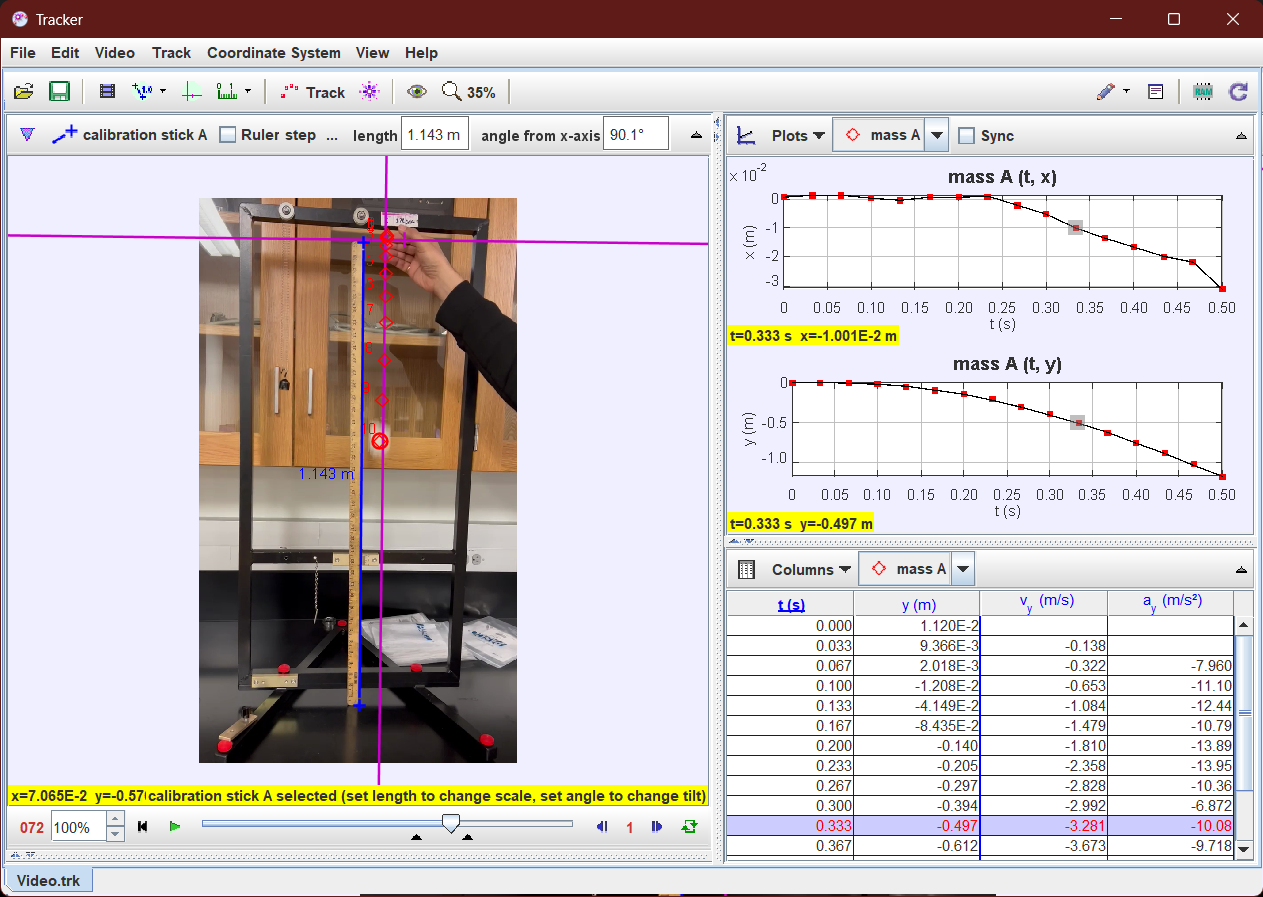
\includegraphics[height=0.7\textheight]{img/trackerSS}
    \caption{Using Tracker\textsuperscript{\textregistered} to analyze the motion of the object.}
    \label{fig:trackerSS}
\end{figure}
\end{frame}

\begin{frame}{Calculating Acceleration}
\begin{columns}
\begin{column}{0.5\textwidth}
   \begin{center}
   \begin{tabular}{|r|r|}
    \hline
    \textbf{Time} \(t\) (s) & \textbf{Y-Position} \(r_y\) (m) \\
    \hline
    0.00E+00 & 1.12E-02 \\
    \hline
    3.33E-02 & 9.37E-03  \\
    \hline
    6.67E-02 & 2.02E-03  \\
    \hline
    1.00E-01 & -1.21E-02 \\
    \hline
    1.33E-01 & -4.15E-02 \\
    \hline
    1.67E-01 & -8.43E-02 \\
	\hline
	\multicolumn{2}{|c|}{\vdots\ \ \ \ \ \ \ \ \ \ \ \ \vdots} \\
	\hline
   \end{tabular}
   \end{center}
\end{column}
\begin{column}{0.5\textwidth}
	\begin{itemize}
		\item \[\vec{v}_{avg,2} = \frac{\vec{r}_3-\vec{r}_1}
				{t_3-t_1}\]
		\item Unlike the last lab, slightly larger time intervals have been
        used to ensure more accuracy.
	\end{itemize}
\end{column}
\end{columns}
\end{frame}

\begin{frame}{Calculating Acceleration}
\begin{columns}
\begin{column}{0.4\textwidth}
    \begin{autotext}
    \begin{itemize}
    \item Repeating this step multiple times, we can get the average
        velocity for each interval
    \item Next step - calculate the acceleration
        \[\vec{a}_{avg,3} = \frac{\vec{v}_4-\vec{v}_2}
				{t_4-t_2}\]
    \end{itemize}
    \end{autotext}
\end{column}
\begin{column}{0.6\textwidth}
	\begin{center}
    \small
    \begin{tabular}{|c|c|c|}
    \hline
    \(t\) (s) & \(r_y\) (m) & \(v_y\) (m) \\
    \hline
    0.00E+00 & 1.12E-02 &  \\
    \hline
    3.33E-02 & 9.37E-03 & -1.38E-01 \\
    \hline
    6.67E-02 & 2.02E-03 & -3.22E-01 \\
    \hline
    1.00E-01 & -1.21E-02 & -6.53E-01 \\
    \hline
    1.33E-01 & -4.15E-02 & -1.08E+00 \\
    \hline
    1.67E-01 & -8.43E-02 & -1.48E+00 \\
    \hline
	\multicolumn{3}{|c|}{\vdots\ \ \ \ \ \ \ \ \ \ \ \ \vdots} \\
	\hline
   \end{tabular}
   \end{center}
\end{column}
\end{columns}
\end{frame}

\begin{frame}{Calculating Acceleration}{Some things to keep in mind}
    \begin{itemize}
	\item Repeating this step multiple times, we can get the average
		acceleration for each interval
	\item Ideally, the average acceleration for each interval should be 
		constant, but due to various factors such as air resistance
		, friction on the surface, etc, the acceleration is not constant. 
	\item Hence, we average the accelerations of these small steps to get an 
	accurate reading.
	\end{itemize}
\end{frame}